\chapter{Umsetzung}
Vorgabe aus der Aufgabenstellung war, das Spiel, das im Rahmen dieses Projekts entwickelt wird, mit der Spieleengine Unity zu entwickeln. Außerdem sollte die Trittfrequenz des Fahrradergometers mittels \textit{Texas Instruments SensorTag} via Bluetooth zur Steuerung des Spiels erfasst werden. Damit war der technologische Rahmen für das Projekt bereits gesetzt.\\
Unity gibt eine relativ klare Struktur für die Umsetzung vor: Es gibt Szenen, in diesen Szenen mehrere Spielobjekte und an diesen dann ein oder mehrere Skripte, die das Verhalten dieses Objektes beeinflussen. Auf die wichtigsten dieser Skripte wird später detailliert eingegangen.\\
Für die Anbindung des Bluetooth-SensorTags erhielten wir von unserem Betreuer eine Android-App, welche die Bluetoothverbindung des Handys nutzt um mit dem Sensor zu kommunizieren, welcher an einem der Pedale befestigt wird. Zusätzlich erfasst das Smartphone die Neigung des Rades. Beide Informationen werden von der App gemeinsam über eine UDP-Verbindung an den Rechner geschickt, auf dem das Spiel läuft. Dieses Zusammenspiel von SensorTag, Smartphone und Spiel wird in Abbildung \ref{Steuerung} dargestellt.\\
\begin{figure}[ht]
\centering
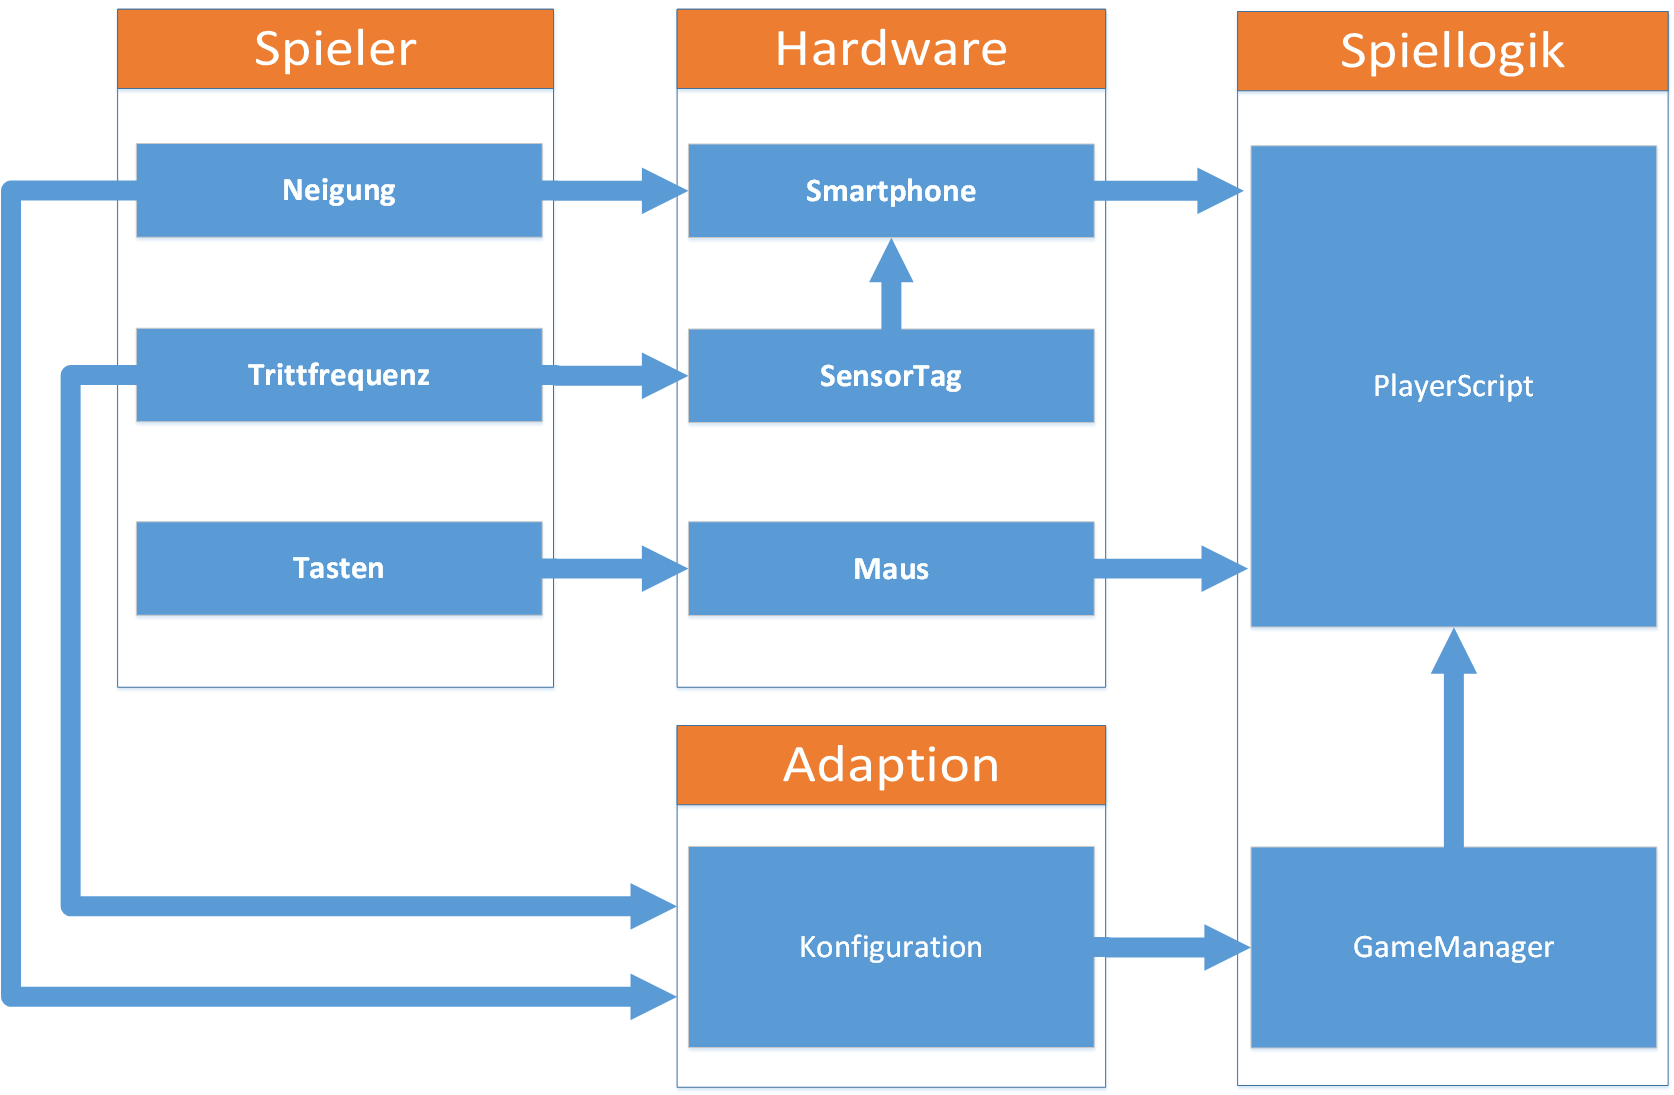
\includegraphics[width=.7\textwidth]{gfx/Steuerung.png}
\caption{Zusammenspiel der verschiedenen Steuerungskomponenten}
\label{Steuerung}
\end{figure}
\section{Steuerung}
Zu den wichtigsten Skripten gehört das \texttt{PlayerScript}. Dieses verarbeitet die verschiedenen Eingaben des Spielers und wandelt diese in Bewegungen um. Je nach Konfiguration wird entweder die Steuerung per Fahrradergometer oder zu Testzwecken die Steuerung per Tastatur verwendet.\\
Die Daten für die Steuerung per Fahrradergometer werden vom \texttt{SensorDataReceiver}-Skript erfasst, indem dieses ein UDP-Socket erstellt, mit dem sich dann das Smartphone verbindet. Das Parsing der Daten erfolgt ebenfalls in diesem Skript.
\section{Leveleditor}
Von Anfang an war klar, dass eine große und abwechslungsreiche Anzahl an Levels für ein gut funktionierendes Spiel wichtig ist. Zuerst war die Idee, diese Levels direkt in Unity als einzelne Szenen zu bauen, doch das erschien uns zu umständlich. Aber selber einen vollständigen Leveleditor zu bauen, hätte wohl den Umfang des Projektes gesprengt.\\
Die Lösung war, einfache Textdateien zu nutzen, und somit einen Texteditor zum Leveleditor zu machen. Die Idee ist dabei, dass jeweils ein Zeichen eine Zelle des Levels füllt. Je nachdem, welches Zeichen dann dort steht, erscheint an dieser Stelle der ein oder andere Baustein, oder es bleibt eine Lücke. Ein Beispiel eines solchen Levels ist in Abbildung \ref{Leveldatei} zu sehen.\\
\begin{wrapfigure}{r}{5.6cm}
\centering
\begin{tabular}{|l|}
\hline
\texttt{25}\\
\texttt{...g...}\\
\texttt{...l...}\\
\texttt{...l...}\\
\texttt{...l...}\\
\texttt{...L...}\\
\texttt{...L...}\\
\texttt{...r...}\\
\texttt{..ftf..}\\
\texttt{...ll..}\\
\texttt{....l..}\\
\texttt{....ll.}\\
\texttt{.....s.}\\
\hline
\end{tabular}
\caption{Beispiel für eine Leveldatei}
\label{Leveldatei}
\end{wrapfigure}
Die Bedeutung der verschiedenen Buchstaben wird im Inspektor des Unity-Editors konfiguriert. Hierbei wird jedem Buchstaben ein Prefab zugewiesen, also ein vorgefertigtes Spielobjekt inklusive eventueller Skripte, die das Verhalten beeinflussen.\\
Ein Buchstabe ohne Zuordnung verursacht dabei keinen Fehler, sondern wird als Lücke interpretiert. Die Konvention ist jedoch, dass nur Punkte für Lücken benutzt werden. Die von uns im Spiel gewählte Zuordnung ist die Folgende:
\begin{itemize}
\item \texttt{l}: Einfacher Streckenabschnitt
\item \texttt{s}: Spieler-Startposition
\item \texttt{g}: Ziel des Levels (Goal)
\item \texttt{t}: Strecke mit Tunnel
\item \texttt{r}: Rampe
\item \texttt{b}: Quadratischer Block in der Mitte des Abschnitts
\item \texttt{f}: Block der über die ganze Breite und Länge des Abschnitts geht
\end{itemize}
Großbuchstaben werden genau wie der entsprechende Kleinbuchstabe behandelt, jedoch wird das Prefab einige Einheiten weiter oben instanziiert, sodass man mittels Klein- und Großbuchstaben Level mit zwei Höhenebenen bauen kann. Die Zahl in der ersten Zeile wird gesondert gelesen und gibt die maximale Leveldauer in Sekunden an.
\section{Szenen}
Auch wenn die einzelnen Level nicht als Szenen realisiert sind, so gibt es dennoch mehrere Szenen im Spiel. Diese sind mit den Szenenübergängen in Abbildung \ref{Szenen} visualisiert.\\
\begin{figure}[ht]
\centering
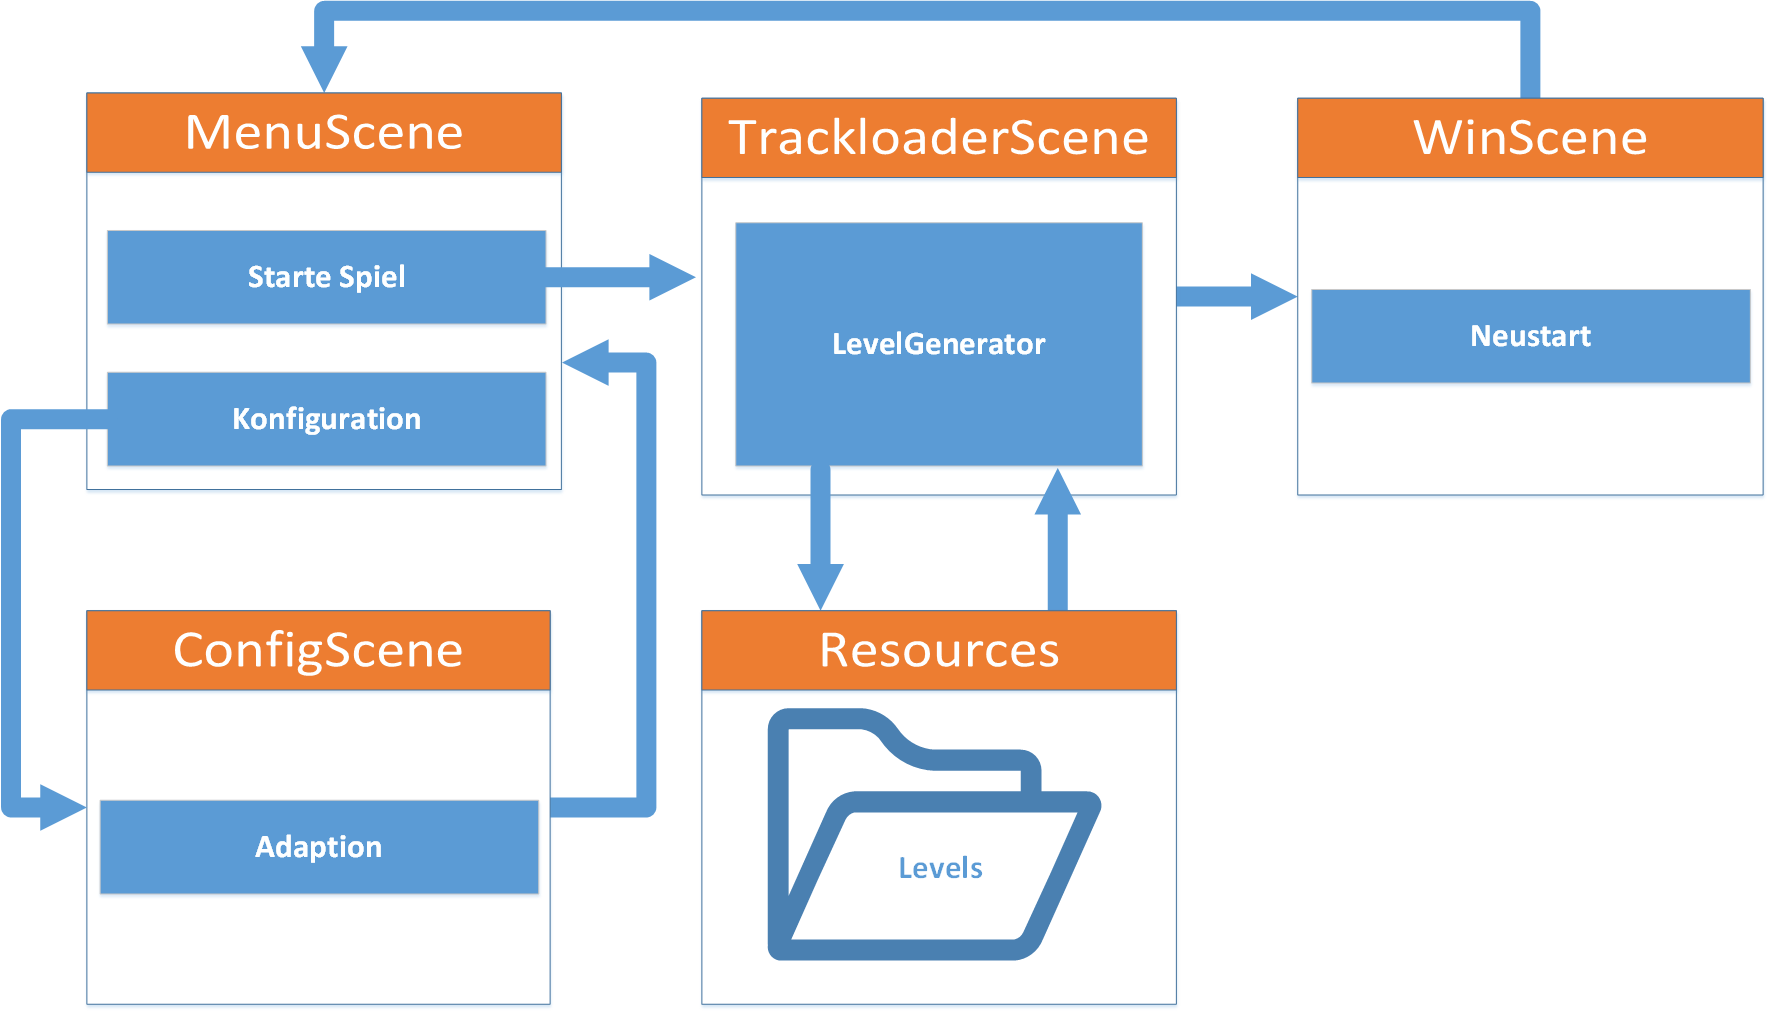
\includegraphics[width=.7\textwidth]{gfx/Szenen.png}
\caption{Szenen und Übergänge}
\label{Szenen}
\end{figure}